% Prof. Dr. Ausberto S. Castro Vera
% UENF - CCT - LCMAT - Curso de Ci\^{e}ncia da Computa\c{c}\~{a}o
% Campos, RJ,  2023 
% Disciplina: An\'{a}lise e Projeto de Sistemas
% Aluno:

\chapterimage{projeto.png} % Table of contents heading image
\chapter{Projeto do Sistema}

Exploraremos a estratégia definida para o desenvolvimento do sistema de gerenciamento de concessionárias de motos. Este projeto é uma parte fundamental na busca por soluções eficazes que aprimorem a administração das concessionárias e a experiência dos clientes. Discutiremos os objetivos do projeto, a metodologia de desenvolvimento, o cronograma, o orçamento e a equipe de projeto. Cada elemento da estratégia é crucial para garantir o sucesso da empreitada e a entrega de um sistema que atenda aos requisitos estabelecidos. Vamos adentrar nas detalhes que direcionarão a realização deste projeto.


\section{Estratégia do Projeto}

O desenvolvimento do sistema de gerenciamento de concessionárias de motos é um projeto crucial que visa fornecer uma solução eficaz e eficiente para melhorar a gestão das concessionárias e aprimorar a experiência dos clientes. A estratégia do projeto é fundamental para garantir o sucesso e a conclusão dentro do escopo, prazo e orçamento definidos.

\subsection{Objetivos do Projeto}

Os principais objetivos do projeto são:

\begin{itemize}
	\item Desenvolver um Sistema Eficiente: O sistema deve ser eficiente e fácil de usar, permitindo que os funcionários da concessionária realizem tarefas de gerenciamento, como cadastro de clientes, registro de vendas e geração de relatórios, de forma simplificada e eficaz.
	
	\item Melhorar a Experiência do Cliente: O sistema deve melhorar a experiência dos clientes, acelerando o processo de compra de motos, fornecendo informações detalhadas sobre os produtos e facilitando o atendimento personalizado.
	
	\item Integração com o Banco de Dados: Garantir que o sistema esteja completamente integrado com o banco de dados que armazena informações sobre clientes, motos e vendas. Isso permite que os dados sejam atualizados em tempo real e fornece uma base sólida para relatórios detalhados.
	
	\item Aprimorar a Gestão de Estoque: O sistema deve fornecer funcionalidades de gerenciamento de estoque para garantir que a concessionária mantenha um controle preciso do inventário de motos disponíveis.
	
	\item Facilitar a Análise de Desempenho: O sistema deve permitir a geração de relatórios detalhados de vendas, fornecendo informações valiosas para análise de desempenho e tomada de decisões.
\end{itemize}

\subsection{Metodologia de Desenvolvimento}

Para a execução deste projeto, adotaremos uma abordagem de desenvolvimento ágil, uma metodologia amplamente reconhecida pela sua eficiência e flexibilidade. Esta abordagem implica na divisão do projeto em iterações, cada uma delas focada em uma funcionalidade específica. Isso permite que as equipes de desenvolvimento trabalhem em colaboração, garantindo que o sistema evolua gradualmente de acordo com as necessidades do usuário.

O processo ágil é caracterizado pela revisão contínua e pela capacidade de fazer ajustes à medida que o projeto avança. Isso significa que estamos preparados para adaptar o sistema às mudanças que possam surgir durante o desenvolvimento, garantindo que ele permaneça alinhado com os requisitos e objetivos do projeto. Essa flexibilidade é fundamental para o sucesso do projeto e a satisfação do cliente, uma vez que permite a incorporação de feedback em tempo real e a entrega de um sistema que realmente atende às necessidades da concessionária e dos clientes.

\subsection{Cronograma}

O projeto seguirá o seguinte cronograma:

O cronograma apresenta um roteiro claro para o desenvolvimento do Sistema de Gerenciamento de Concessionárias de Motos, detalhando as atividades ao longo das 37 semanas do projeto.

\begin{figure}[h]
	\centering
	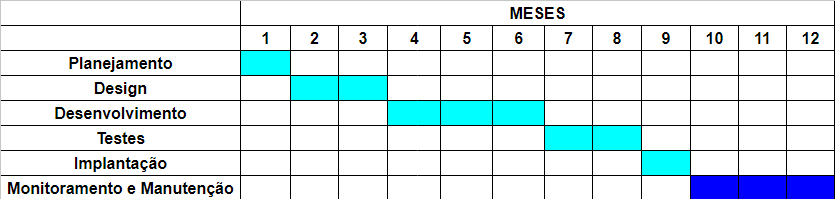
\includegraphics[width=\textwidth]{cronograma.png}
	\caption{Cronograma do Projeto}
	\label{fig:cronograma}
\end{figure}

Planejamento de atividades ao longo das próximas semanas, fornecendo uma visão abrangente do cronograma do projeto.
\begin{enumerate}
	\item Fase de Planejamento (Duração: 4 semanas)
	\begin{itemize}
		\item Identificação de Requisitos e Análise de Necessidades (2 semanas)
		\item Definição de Escopo e Objetivos (1 semana)
		\item Elaboração do Plano de Projeto (1 semana)
	\end{itemize}
	
	\item Fase de Design (Duração: 6 semanas)
	\begin{itemize}
		\item Design da Interface do Usuário (2 semanas)
		\item Arquitetura de Software e Banco de Dados (2 semanas)
		\item Especificações Técnicas (2 semanas)
	\end{itemize}
	
	\item Fase de Desenvolvimento (Duração: 12 semanas)
	\begin{itemize}
		\item Desenvolvimento do Software (8 semanas)
		\item Testes Unitários (2 semanas)
		\item Integração de Módulos (2 semanas)
	\end{itemize}
	
	\item Fase de Testes (Duração: 8 semanas)
	\begin{itemize}
		\item Testes de Aceitação do Usuário (4 semanas)
		\item Testes de Desempenho (2 semanas)
		\item Correções e Ajustes (2 semanas)
	\end{itemize}
	
	\item Fase de Implantação (Duração: 4 semanas)
	\begin{itemize}
		\item Treinamento de Usuários (2 semanas)
		\item Preparação para Lançamento (1 semana)
		\item Implantação do Sistema (1 semana)
	\end{itemize}
	
	\item Fase de Monitoramento e Manutenção (Duração: Contínua após a implantação)
	\begin{itemize}
		\item Suporte Técnico (em curso)
		\item Atualizações de Software (em curso)
		\item Monitoramento de Desempenho (em curso)
	\end{itemize}
	
\end{enumerate}

\subsection{Orçamento}

O orçamento para este projeto inclui custos de desenvolvimento de software, custos de treinamento e despesas operacionais. O orçamento total estimado é de R\$ 200.000.

\subsection{Equipe do Projeto}

A equipe do projeto é composta por desenvolvedores de software, analistas de negócios, gerentes de projeto e especialistas em banco de dados. Cada membro da equipe desempenha um papel vital na concepção, desenvolvimento e implementação do sistema.

A estratégia do projeto estabelecida visa cumprir os objetivos e fornecer um sistema de alta qualidade que atenda às necessidades das concessionárias e clientes. A próxima seção abordará os requisitos detalhados do sistema.

\section{Refinamento dos Diagramas DFD e E-R}

Nesta seção, realizaremos o refinamento dos Diagramas de Fluxo de Dados (DFD) e dos Diagramas de Entidade-Relacionamento (E-R) que descrevem o processo de venda na concessionária de motos. Essas representações visuais são essenciais para compreender e aprimorar o processo, facilitando o desenvolvimento do sistema que atenderá às necessidades dos funcionários da concessionária e dos clientes.

\subsection{Refinamento do Diagrama DFD}

Os DFDs são ferramentas essenciais para visualizar e analisar o fluxo de informações e as interações envolvidas em cada etapa do processo de venda. Começaremos refinando os DFDs.




\subsubsection{DFD de Alto Nível - Processo de Venda}

O DFD de alto nível representa o processo de venda de forma simplificada, destacando os principais atores e fluxos de dados. Este DFD é uma visão geral do processo e inclui os seguintes elementos:

\begin{itemize}
	\item \textbf{Funcionário da Concessionária}: Este ator inicia o processo de venda e interage diretamente com o cliente.
	\item \textbf{Atendimento ao Cliente}: Representa a interface do cliente no processo de venda.
	\item \textbf{Dados do Cliente}: Este fluxo de dados contém informações pessoais do cliente, como nome, endereço e informações de contato.
	\item \textbf{Informações sobre Motos Disponíveis}: Inclui detalhes sobre as motos disponíveis no estoque, como marca, modelo, ano, preço e especificações.
	\item \textbf{Registro de Venda}: Representa o registro das informações relacionadas à venda, incluindo a data da transação e os detalhes das motos vendidas.
\end{itemize}

O DFD de alto nível fornece uma compreensão geral do processo de venda, mas agora nos aprofundaremos em detalhes com DFDs mais específicos.

\subsubsection{DFD Detalhado - Processo de Venda}

O DFD detalhado expande cada etapa do processo de venda em maior profundidade. Vamos destacar as principais funcionalidades em cada parte do processo:

\paragraph{Atendimento ao Cliente}

Nesta etapa, o "Funcionário da Concessionária" inicia a interação com o cliente, que é representado pelo "Atendimento ao Cliente." Os principais fluxos de dados incluem:

\begin{itemize}
	\item \textbf{Identificação de Necessidades}: O funcionário coleta informações sobre as necessidades do cliente em relação à compra da moto.
	\item \textbf{Requisitos do Cliente}: São os critérios do cliente, como preferências de marca, modelo e outras especificações.
\end{itemize}

\paragraph{Apresentação das Motos Disponíveis}

Nesta etapa, o funcionário apresenta as motos disponíveis que atendem às necessidades do cliente. Os principais fluxos de dados são:

\begin{itemize}
	\item \textbf{Informações Detalhadas das Motos}: Isso inclui os detalhes das motos disponíveis, como marca, modelo, ano, preço e especificações técnicas.
	\item \textbf{Seleção da Moto pelo Cliente}: Representa a escolha do cliente em relação à moto desejada.
\end{itemize}

\paragraph{Registro dos Dados do Cliente}

Se o cliente decidir prosseguir com a compra, o funcionário registra os dados pessoais do cliente. Os fluxos de dados incluem:

\begin{itemize}
	\item \textbf{Informações do Cliente}: Inclui dados como nome, endereço e informações de contato do cliente.
	\item \textbf{Confirmação da Compra}: Indica que o cliente está comprometido com a compra da moto.
\end{itemize}

\paragraph{Registro da Venda}

Nesta etapa final, o funcionário registra a venda, incluindo os detalhes da moto vendida e a data da transação. Os principais fluxos de dados são:

\begin{itemize}
	\item \textbf{Detalhes da Venda}: Inclui informações como preço final, data da venda e outros detalhes financeiros.
	\item \textbf{Estoque Atualizado}: Reflete as mudanças no estoque da concessionária após a venda.
\end{itemize}

\begin{figure}[h]
	\centering
	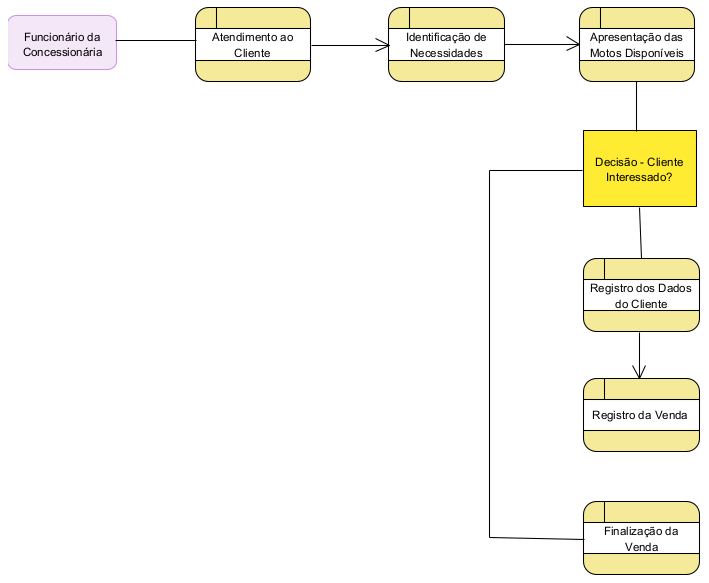
\includegraphics[width=0.7\textwidth]{diagrama-vendas.png}
	\caption{Diagrama de Fluxo de Dados}
	\label{fig:Diagrama de Fluxo de Dados}
\end{figure}

\subsubsection{Conclusão}

O refinamento dos Diagramas de Fluxo de Dados fornece uma visão mais detalhada do processo de venda na concessionária de motos. Essas representações visuais são essenciais para compreender e aprimorar o processo, facilitando o desenvolvimento do sistema que atenderá às necessidades dos funcionários da concessionária e dos clientes.

\subsection{Refinamento do Diagrama Entidade-Relacionamento (E-R)}

Nesta seção, iremos aprimorar o Diagrama Entidade-Relacionamento (E-R) para modelar as entidades Cliente, Venda e Moto, juntamente com seus atributos e relacionamentos.



\subsubsection{Entidades}

\paragraph{Cliente}

A entidade "Cliente" representa as informações dos clientes da concessionária de motos. Ela possui os seguintes atributos:

\begin{itemize}
	\item \textbf{IDCliente}: Identificador único para cada cliente.
	\item \textbf{Nome}: Nome do cliente.
	\item \textbf{Idade}: Idade do cliente.
	\item \textbf{Telefone}: Número de telefone do cliente.
	\item \textbf{Email}: Endereço de e-mail do cliente.
	\item \textbf{Endereço}: Endereço do cliente.
\end{itemize}

\paragraph{Venda}

A entidade "Venda" registra informações sobre cada venda realizada na concessionária. Seus atributos incluem:

\begin{itemize}
	\item \textbf{IDVenda}: Identificador único para cada venda.
	\item \textbf{DataCompra}: Data em que a venda foi realizada.
	\item \textbf{IDCliente}: Uma chave estrangeira que se relaciona com a entidade "Cliente," indicando o cliente envolvido na venda.
	\item \textbf{IDMoto}: Uma chave estrangeira que se relaciona com a entidade "Moto," indicando a moto vendida.
\end{itemize}

\paragraph{Moto}

A entidade "Moto" contém informações sobre as motos disponíveis na concessionária. Seus atributos são:

\begin{itemize}
	\item \textbf{IDMoto}: Identificador único para cada moto.
	\item \textbf{Modelo}: Modelo da moto.
	\item \textbf{Ano}: Ano de fabricação da moto.
	\item \textbf{Preço}: Preço da moto.
	\item \textbf{Cor}: Cor da moto.
\end{itemize}

\subsubsection{Relacionamentos:}


\paragraph{Relacionamento entre Cliente e Venda}

Há um relacionamento entre a entidade "Cliente" e "Venda," com uma cardinalidade de 1 para N, o que significa que um cliente pode estar associado a várias vendas, mas cada venda está relacionada a apenas um cliente. Este relacionamento é representado por uma chave estrangeira "IDCliente" na entidade "Venda."

\paragraph{Relacionamento entre Venda e Moto}

Há um relacionamento entre a entidade "Venda" e "Moto," também com uma cardinalidade de 1 para N. Isso significa que uma venda pode incluir várias motos, mas cada moto está associada a apenas uma venda. Este relacionamento é representado pela chave estrangeira "IDMoto" na entidade "Venda."

\begin{figure}[h]
	\centering
	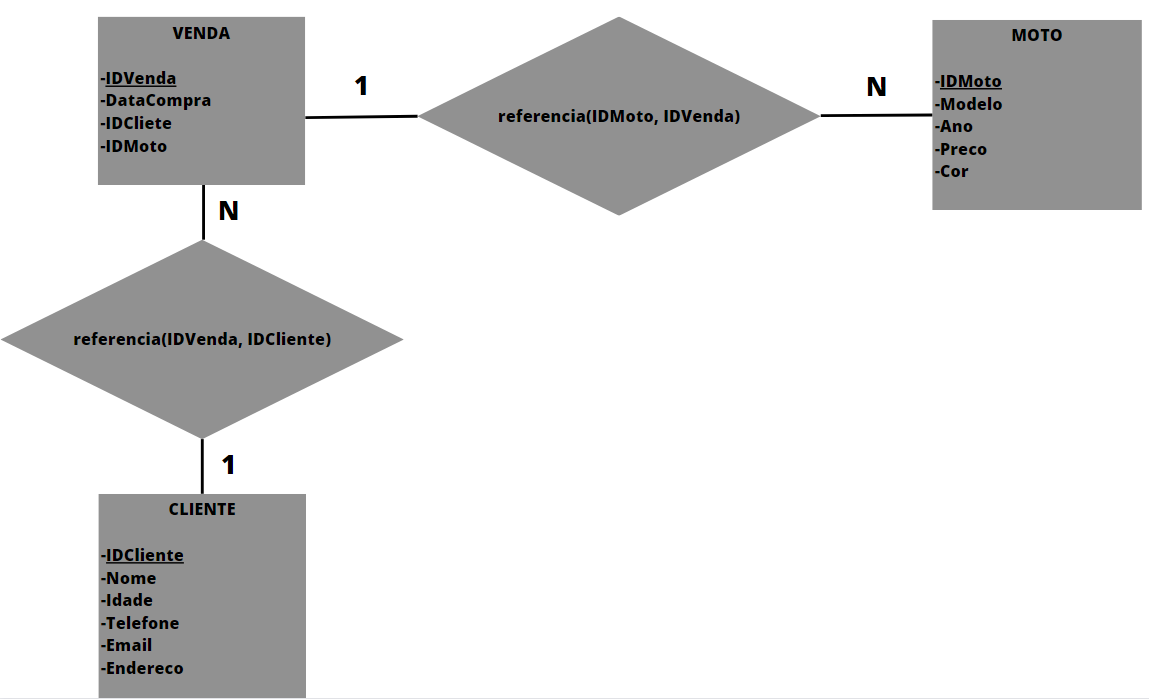
\includegraphics[width=0.7\textwidth]{banco-de-dados.png}
	\caption{Diagrama de Entidade-Relacionamento (E-R)}
	\label{fig:Diagrama de Banco de Dados}
\end{figure}

\subsubsection{Conclusão}

O refinamento do Diagrama Entidade-Relacionamento proporciona uma representação visual mais detalhada das entidades, atributos e relacionamentos do sistema de gerenciamento de concessionárias de motos. Isso auxiliará no desenvolvimento do banco de dados e na compreensão das interações entre os componentes do sistema.


\section{Arquitetura do Sistema - Estilos}


    \subsection{Arquitetura do Sistema}

\begin{figure}[h]
	\centering
	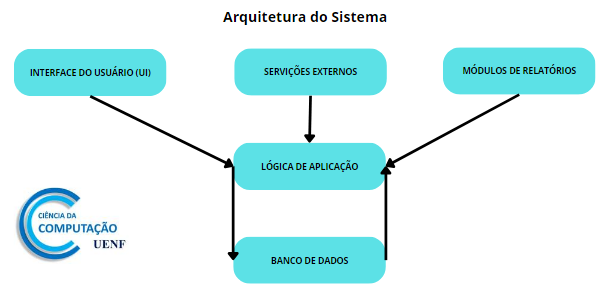
\includegraphics[width=\textwidth]{diagrama1.png}
	\caption{Arquitetura do Sistema}
	\label{fig:diagrama1}
\end{figure}

Neste exemplo, as setas indicam que o Cliente envia solicitações para o Servidor de Aplicação, que, por sua vez, interage com o Banco de Dados para buscar ou modificar informações. As setas indicam a direção do fluxo de comunicação entre os componentes, e representam a troca de informações ou requisições entre os componentes.

\subsubsection{Cliente}

O componente Cliente representa as interfaces de usuário, como aplicativos móveis ou navegadores, que interagem diretamente com o sistema. Ele envia solicitações para o Servidor de Aplicação e exibe as informações recebidas aos usuários.

\subsubsection{Servidor de Aplicação}

 O Servidor de Aplicação é responsável por processar as solicitações dos clientes, gerenciar a lógica de negócios e coordenar as interações com o Banco de Dados. Ele recebe as requisições do Cliente, realiza operações necessárias e envia as respostas de volta.

\subsubsection{Banco de Dados}

O Banco de Dados armazena e gerencia os dados do sistema. Ele recebe instruções do Servidor de Aplicação para recuperar, modificar ou adicionar informações. Isso garante a persistência e integridade dos dados do sistema.


    \subsection{Arquitetura do Hardware}

\subsubsection{Servidor Web}

\textbf{Descrição:} Responsável por hospedar e servir a aplicação web. \\
\textbf{Hardware:} Servidor físico de alta capacidade. \\
\textbf{Software:} Servidor web (por exemplo, Apache, Nginx).

\subsubsection{Servidor de Banco de Dados}

\textbf{Descrição:} Armazena e gerencia os dados da aplicação. \\
\textbf{Hardware:} Servidor dedicado para banco de dados. \\
\textbf{Software:} Sistema de gerenciamento de banco de dados (por exemplo, MySQL, PostgreSQL).

\subsubsection{Dispositivo de Cliente}

\textbf{Descrição:} Dispositivo usado pelos usuários para acessar a aplicação. \\
\textbf{Hardware:} Pode ser um computador, laptop, tablet ou smartphone. \\
\textbf{Software:} Navegador web para acessar a aplicação.

\subsubsection{Conexões}

\begin{itemize}
	\item O Dispositivo de Cliente se conecta ao Servidor Web para acessar a aplicação.
	\item O Servidor Web se conecta ao Servidor de Banco de Dados para recuperar ou armazenar dados necessários.
\end{itemize}

\subsubsection{Fluxo de Dados}

\begin{itemize}
	\item O Cliente faz uma solicitação ao Servidor Web para acessar a aplicação.
	\item O Servidor Web processa a solicitação e, se necessário, interage com o Servidor de Banco de Dados para obter dados.
	\item O Servidor Web envia a resposta de volta ao Cliente.
\end{itemize}

\begin{figure}[h]
	\centering
	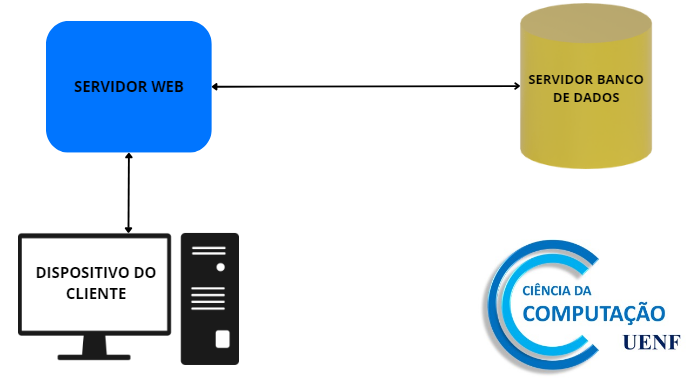
\includegraphics[width=\textwidth]{diagrama2.png}
	\caption{Arquitetura do Hardware}
	\label{fig:diagrama1}
\end{figure}


    \subsection{Arquitetura de Software}

O diagrama de software apresenta a estrutura fundamental do Sistema de Gerenciamento de Concessionária de Motos, destacando os principais componentes de software e suas interações. A seguir, descrevemos cada componente:

\begin{itemize}
	\item \textbf{Sistema de Gerenciamento de Concessionária de Motos:} Representa o sistema como um todo, englobando todas as camadas.
	
	\item \textbf{Aplicação Web (Frontend):} Responsável pela interface do usuário, proporcionando uma experiência interativa. Utiliza tecnologias como HTML, CSS, JavaScript, React, Angular, entre outras.
	
	\item \textbf{Servidor de Aplicação (Backend):} Gerencia a lógica de negócios e processa as solicitações do cliente. Implementado com tecnologias como Node.js, Django, Flask, Spring, entre outras.
	
	\item \textbf{Banco de Dados:} Armazena e gerencia os dados do sistema, garantindo persistência. Utiliza um sistema de gerenciamento de banco de dados (SGBD) como MySQL, PostgreSQL, ou outro.
\end{itemize}

\begin{figure}[h]
	\centering
	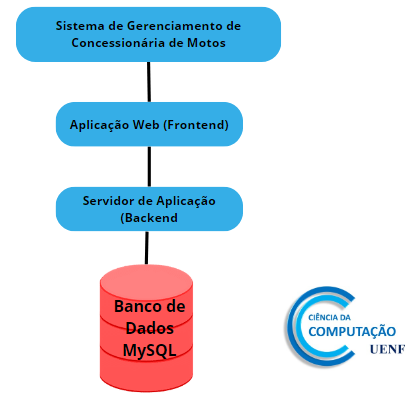
\includegraphics[width=\textwidth]{diagrama3.png}
	\caption{Arquitetura de Software}
	\label{fig:diagrama1}
\end{figure}
